%%% This LaTeX source document can be used as the basis for your technical
%%% report. Intentionally stripped and simplified
%%% and commands should be adjusted for your particular paper - title, 
%%% author, citations, equations, etc.
% % Citations/references are in report.bib 

\documentclass[conference]{acmsiggraph}

\usepackage{graphicx}
\graphicspath{{./images/}}
\newcommand{\figuremacroW}[4]{
	\begin{figure}[h] %[htbp]
		\centering
		\includegraphics[width=#4\columnwidth]{#1}
		\caption[#2]{\textbf{#2} - #3}
		\label{fig:#1}
	\end{figure}
}

\newcommand{\figuremacroF}[4]{
	\begin{figure*}[h] % [htbp]
		\centering
		\includegraphics[width=#4\textwidth]{#1}
		\caption[#2]{\textbf{#2} - #3}
		\label{fig:#1}
	\end{figure*}
}


\usepackage{lipsum}

\TOGonlineid{45678}
\TOGvolume{0}
\TOGnumber{0}
\TOGarticleDOI{1111111.2222222}
\TOGprojectURL{}
\TOGvideoURL{}
\TOGdataURL{}
\TOGcodeURL{}

\title{Performance Analysis of Real Time Multi-platform Physics Simulations \\
	   Design Document}

\author{Sam Serrels\\\ 40082367@napier.ac.uk \\
Edinburgh Napier University\\
Physics-Based Animation (SET09119)}
\pdfauthor{Sam Serrels}

\keywords{Multi-platform Physics, Optimisation, GPU, Cell, PS3}

\begin{document}

\teaser{
   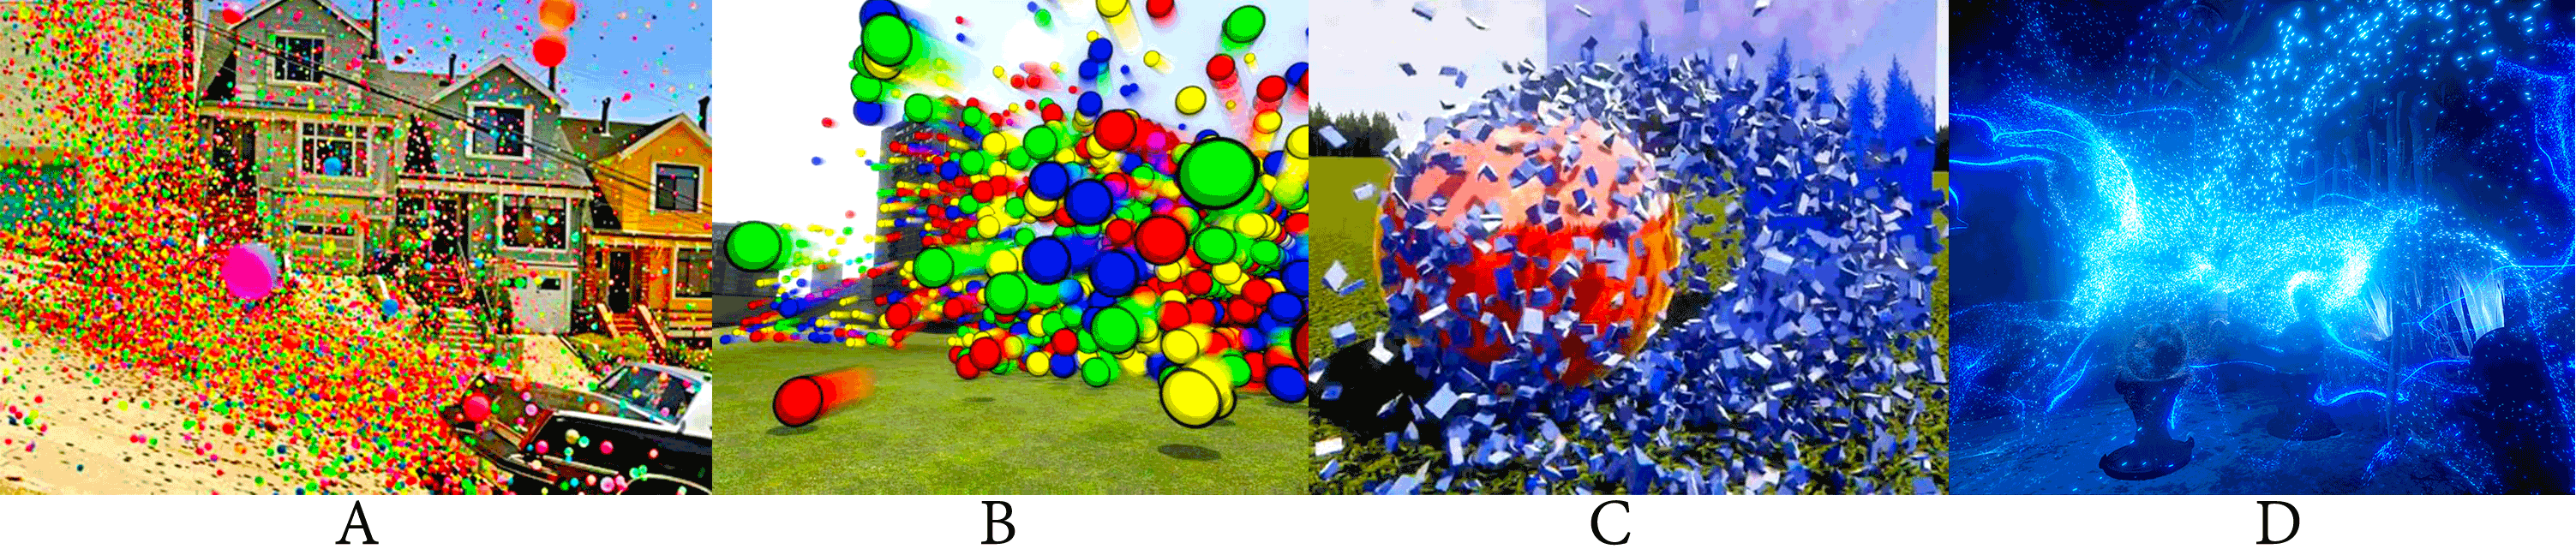
\includegraphics[height=1.5in]{images/sampleteaser}
   \caption{A) Project Inspiration \protect\cite{advert}, (B) Rigid bodies \protect\cite{gmod}, (C) Colliding Particles \protect\cite{cryengine}, (D) Non colliding particles \protect\cite{ue4}}   
 }

\maketitle

\begin{abstract}
This project aims to develop a physics engine and simulate a scene consisting of thousands of bouncing balls, running on various systems, such as the Sony Playstion 3.
the performance of each system will be measured as the systems are optimised and will be compared in the final report.
\end{abstract}

\keywordlist
%\copyrightspace

\section{Introduction}

Realistic Real time physics simulation is highly sought after in interactive applications, especially games. Achieving high-accuracy while maintaining performance in often resource restricted environments(I.E a games console) requires the highest level of optimisations and often results in a trade-off with simulation speed against Accuracy. This project attempts to record and analyse the performance of various optimisations on a simulated scene. This will be taken further by applying the project to various different processing architectures. The scene that will be simulated is a large set of Bouncy balls, travelling down a hill.

\paragraph{Physics Engines}
Large and complex video games tend to use 3rd party physics solutions, this vastly cuts down on the project development man-hours, and the maintenance thereafter. Third party physics solutions have the benefit of being battle tested out in the wild beforehand, so internal reliability is usually a given. A further benefit is that being developed solely for the purpose of being a "a good physics engine" by people who are usually experts in the field, large optimisations are already implemented. The problems arise in the implementation, the coupling of a physics engine and the existing codebase. While they are usually well coded, they are not tailor made to each game. 

\paragraph{Optimising for Physics Engines}
Trying to regain performance from an external physics engine can be a hard task, diving into the source code requires expert knowledge of the inner-workings of the whole system. A common path is to shape the design of the game code to conform better to the demands of the physics engine and hope that the internal optimisations  will be sufficient. Often enough, they are not.

\paragraph{Shipping on consoles}
Video games consoles have vastly varying hardware capabilities and architecture, writing robust code that is performant on all of them is a rarely possible. Code has to be re-designed for each system. The simple truth: more code means more problems, so throwing a large complex physics engine that you have no knowledge of the inter-working of into the mix, is a recipe for bad performance and bad code. However some physics systems do have separate versions for different architectures, assuming the interface is unchanged, games can swap in different libraries at compile-time. A further extension on to this would be to abstract all the physics so many different libraries can be plugged in.

\paragraph{Project Aims}
This project will attempt to create a physics solution that will run on various systems, along with a game engine with an appropriate interface to swap in other existing physics solutions. This will allow for fair comparisons and benchmarking of the physics solution created by this project.\\
The target platforms will be the Sony Playstation 3, Sony Playstation Vita and a conventional x86 multi-core PC architecture.
Utilising the general purpose processing functionality of the graphics cards within the PC system for physics is also a possibility.

\paragraph{Project Application}
The systems created in the project will be used to simulate a demo scene, picked to be processing intensive. The scene will be a large set of bouncy balls, bouncing down a sloped street. This will result in plenty of collisions, a large amount of data needing transferred every frame, and something interesting to watch. The inspiration for this came from a Tv advert \cite{advert} where a similar thing was filmed in reality, with real bouncy balls and a real street.

\paragraph{Lack of Statistics}
Developers who make physics engines written and optimised for a single specific game don't usually publish much information on the performance. The results are always relative the specific game and have little meaning when applied to any other project. General Physics optimisations and platform specific optimisation methods are published, but are rarely included with performance statistics. This project aims to have a breakdown of all the optimisations taken with numerical performance statistics.

\section{Related Work}

\figuremacroF
{bullet}
{Bullet Physics PS3 Pipeline}
{Requires Intermediate Data Swapping Between PPU and SPU \protect\cite{spuphys}}
{0.96}
\figuremacroF
{insomniac}
{Insomniac Physics Pipeline}
{No Intermediate Data Swapping Between PPU and SPU once the physics job has started \protect\cite{spuphys}}
{0.96}

\paragraph{Physics on the PS3}
Some of the major physics libraries have been ported in some fashion to the Playstation 3.
\begin{description}
  \item[Havok] \hfill \\
   The Havok physics engine is the most widely used 3rd party library for custom game engines and larger engines such as Unreal Engine 3. The library is a proprietary  technology and information regarding the specific PS3 implementation is not publicly available.
  \item[Physx] \hfill \\
  The Nvidia Physx sdk was ported to the PS3, but it's use in released games is mostly undocumented. The PS3's "RSX" GPU does not include the CUDA architecture that modern Gpus use to further accelerate Physics.
  \item[Bullet] \hfill \\
  A fork of the open source physics engine "Bullet", was developed and released. Although not a popular PS3 engine, shipping with only a handful of games, it served mainly as a reference for other engines. As of 2012 this is no longer in active development.
\end{description}

\paragraph{Custom engines}
Unfortunately there is no good statistics on the ratio of games shipped with custom physics engines versus 3rd party physics. 
Documentation and relevant publications on the subject are also rare, the most documented physics implementations are the Bullet engine and the custom engine made by Insomniac games.

\paragraph{Insomniac's approach}

Insomniac games developed a custom solution for utilising the Playstations's SPUs as efficiently as possible, called SPU Shaders. Although not actually linked to shading or rendering, they follow a similar design to graphics shaders, by being modular self contained modules with one specific purpose.\\
Formally defined as:
\begin{quote}
\begin{itemize}
  \item Fragments of code used in a larger system
  \item Code is injected at location pre-determined by
system.
  \item Custom made for any particular system.
  \item Allows modifications of system data.
  \item Can feedback to other systems outside the scope of the current system.
\end{itemize}
\cite{spushaders}
\end{quote}

This system is used extensively for all SPU work in the game, but is also key the implantation of the physics engine. This allows for a modular physics system, tailor made to the SPU's limitations and strengths. The primary benefit is that it also becomes a standalone set of tasks, leaving the main processing thread to deal with other tasks.
(See Fig:\ref{fig:insomniac})

\paragraph{Bullets's approach}
The Bullet PS3 implementation took more of a \textit{port} approach rather than a \textit{complete redesign}. This makes sense as Bullet is a Library rather than a single game solution, effort was made to keep the core codebase as untouched as possible to allow for greater stability across all the platforms. The main work was done in the area of scheduling and threading. The system was designed so that the SPU jobs could easily be reimplemented on another platform like the Xbox360 as CPU threads. The SPU code had it's major specific changes in the region of data management and loading, the physics processing code remains largely unchanged apart from some minor optimisations.
\begin{quote}
``The Generic convex collision algorithm performs a bit less then specific algorithms.\\
This generic approach requires Intermediate Data Swapping Between PPU and SPU and requires synchronization between SPUs''
\cite{spuphys}
\end{quote}
(See Fig:\ref{fig:bullet})

\paragraph{Physics on the Vita}
the Processing architecture of the Playstation Vita is similar to that of a common desktop processor with 4 cores, the difference being that the instruction set is ARM rather than X86. The gpu is designed for graphics, and graphics only, so all physics processing on the vita will take place on the GPU. At the current time the only documented Physics library for the Vita is Havok, with no public published articles regarding performance or implementation details. 

\paragraph{Physics on the PC}
There are multitudes of different physics implementations on the traditional architecture of the PC, where the extra resources of the hardware mean that more focus can be placed on usability and implementation of the physics. It is more common to see physics engines compared against each other based on the complexity of the code rather than the runtime performance (this is also partly to do with the large hardware and capability differences between computer systems). Many reports have been published analysing the software design methodologies and ease of implementation of physics engines. 
\begin{quote}
``Using Software Quality Metrics which give an empirical indication of (among other
things) the reusability, usability, and flexibility of a piece of software—we can begin to
investigate ways of improving the games development process.''\cite{comparison}
\end{quote}

\paragraph{This project}
This project will take a similar approach to that of Bullet, by creating a generic physics engine that will run on multiple systems with as little as modification as possible, while still aiming for the best performance. The end result should be a program that uses good software design methodologies, meaning code that is easy to understand and modify. Platform specific modification can then be implemented and the change in performance against the change in code complexity can be measured.

\section{Simulation}

\paragraph{Scope of Physic capabilities}
The physics engine created for this project will be limited in scope and capabilities rather than a full general solver. The primary function will be Collision detection and realistic movement of single rigid-bodies. Constraints, animation, Inverse Kinematics, and advanced mass calculations are not planned to be implemented although the system should be designed to accommodate these systems in the future.

\paragraph{Simulation Scene}
The project will be simulating a large set of bouncing balls travelling down a hill. The ball will be solid object with mass, and will collide with each other and the surrounding geometry. the geometry will consist of flat shaded primitive shapes, to roughly emulate the real life scenery of the street in the advert.

\paragraph{Simulation Objectives}
The aim of the simulation is to measure the performance of the physics simulation, I.e the maximum amount of balls that can be simulated. Rendering the scene is also an objective, as a physics simulation that cannot be rendered, either by design or by taking up too many resources is of no use for a real-time application.

\paragraph{Simulation Variables}
The balls will be created somewhat randomly, to the simulation should look different every time it is run. Variables could include changing the size and bounciness e of the balls, changing the design of the environment (street slope, length, frequency of objects... ) and other physics variables, like time-step and gravity.

\paragraph{Rendering}
Rendering the output of the simulation should result in a visually interesting scene, hopefully as similar to the reference video as possible. The focus of this project is optimising the simulation, but an impressive looking output that also achieves a good level of performance (60+fps) would be a large bonus to the project.

\paragraph{Data output}
The simulations should be logging and metering all the data to file as well as rendering the scene, this will be used in the evaluation report.

\section{Application Description}

\figuremacroW
{balls2}
{Expected visualisation of the output}
{Background geometry will not be this detailed \protect\cite{advert}}
{0.96}

The scene will start with an initial amount off balls at the top of the hill. They will be dropped from a height or fired via some force to give them initial velocity. Over time more ball will be created at the top of the hill to keep the simulation going. Balls may be removed once they reach the bottom of the hill or after a set time, this will depend on the overall performance limitations.

\paragraph{User Interaction}
The user will be able to use the input controls to move the camera around in the scene, to get close up views of whatever they choose. There will also be controls to alter the variables in the scene and execute gameplay functions. Input methods will take the form of a controller / mouse and keyboard where applicable.

\paragraph{Gameplay functions}
Functions that the user can use could include: adding forces to the scene, adding groups of balls at a certain location, removing balls, firing balls, and resetting the simulation.

\section{Technical Specification}

\paragraph{Parallelism}
the key to success in implementing this project will be to heavily rely on multi-core/multi-thread/multi-processor software architecture. For the Playstation 3 this is an absolute necessity, as the SPUs are the only obvious way to implement physics. A parallel approach will benefit all systems, and designing for the small memory limits of the SPU will also benefit other platforms as smaller code and datasets can make use of the extensive caching available on Desktop Processors.

\begin{quote}
``Old Processing model: Big semi truck. Stuff everything in. Then stuff some
more. Then put some stuff up front. Then drive
away.\\
New SPU model: Fleet of Ford GTs taking off every five minutes.
Each one only fits so much. Bucket brigade. Damn they're fast!''
 \cite{spuspeed}
\end{quote}

\paragraph{Optimisation}
Optimisation can be split into 2 large categories, algorithmic optimisations and data optimisations. Algorithmic optimisations is the process of monitoring all the operations done within a physics tick to spot redundant operations, or to swap slow operations for faster methods. This can be done initially by using profiling, but it can result in going down to the compiled assembler code to see if the compiler is misbehaving. This is often the case when trying to squeeze every process cycle out of an SPU due to it's highly vectorised SIMD based instruction set.

\paragraph{Data Optimisation}
This is the task of minimizing the transference and duplication of data. Moving Data takes time and can hog buses and caches that need to be used by other systems.
In a panellised systems this can become a headache as the extra case of \textit{when} items need to be accessed needs to be take into account, so that threads are not blocked by other threads.

\paragraph{Achieving Optimisation}
This project intends to measure the very best performance out of the different systems, getting to that level of performance will take a large amount of the development time. Real-world game projects have resource budgets and target to hits (i.e 60fps) and then they can ship the game. This project has no performances target, so the aim is to keep optimising until there is nothing left to optimise.

\paragraph{Software Design}
The project will be written as one solution with platform modules automatically swapped at compile time, rather than a separate project for each solution. this promotes shared code between the systems which reduces bugs and increases code quality. This method does have the downside of possibly having a large maze of "\#ifdefs" but with proper inheritance and code design, the impact should be minimal an confined only to the interface classes.

\paragraph{Physics abstraction}

In this section, you should put together some of the technical details of your simulation.  This will help when developing your physics-based simulation later.

\paragraph{External libraries}
The current list of libraries that project will require is as follows:
\begin{description}
  \item[SDL - Simple DirectMedia Layer] \hfill \\
  	Used for creating windows, polling input and general useful platform code for PC/mac/linux.
  \item[GLEW -  The OpenGL Extension Wrangler Library] \hfill \\
  	Used as the entry point into the OpenGl framework, used for detecting graphics capabilities.
  \item[GLM -  OpenGL Mathematics] \hfill \\
  	Maths Library used on Pc platforms.
\end{description}


\section{Conclusion}
In conclusion, this project should generate some new information about the physics capabilities of the Playstation 3 and Plystation Vita, along with an interesting interactive display of the simulation.


% \section*{Acknowledgements}


\bibliographystyle{acmsiggraph}
\bibliography{report}

\end{document}

